\subsection{Ergebnisse}
Das Kapitel der Ergebnisse befasst sich mit der konkreten Umsetzung der gesamten Applikation und dokumentiert die grundlegenden Ergebnisse oder Resultate, welche aus dieser Arbeit hervorgegangen sind. 

Auch hier soll nochmals erwähnt sein, dass diese Arbeit auf der Studienarbeit \cite{methode635-sa} aufbaut und grundlegende Informationen dort nachzulesen sind. 

In diesem Kapitel gehen wir zunächst auf die Änderungen während der Refactoring-Phase ein und schildern was dies für die Wartung und Erweiterung des Codes bedeutet. 

Anschliessend sind weitere Features dokumentiert, welche im Verlauf dieser Arbeit an der Applikation durchgeführt wurden.

Das Kapitel wird durch eine Gegenüberstellung der erreichten und geplanten Arbeit abgeschlossen.

Zur besseren Übersicht wurde der Code vereinzelt gekürzt. Dies ist durch 3 Punkte (...) gekennzeichnet.

\subsubsection{Refactoring zu Beginn der Arbeit}
Wie aus dem Projektplan (siehe Abbildung \ref{fig:projekt-plan}) zu entnehmen ist, haben wir uns zu Beginn unserer Arbeit dazu entschieden, zwei Sprints für das Refactoring unsere Applikation zu nutzen. Die Entscheidung überhaupt ein Refactoring durchzuführen entstand aus der Tatsache, dass wir schon gegen Ende der Studienarbeit gemerkt hatten, dass bei einer allfälligen Weiterführung der Arbeit ein Refactoring von grossem Wert sein wird. Auch haben wir diesbezüglich schon während der Studienarbeit einzelne Vorschläge für ein Refactoring beschrieben.


Das Ziel der Refactoring-Phase war es daher, den Code, welcher aus der Studienarbeit hervorgegangen ist, zu prüfen und zu verbessern. Dies sollte uns helfen, die Erweiterbarkeit für zukünftig geplante Features zu gewähren.

Auch konnten wir die in der Studienarbeit beschriebenen Vorschläge erfolgreich in der App umsetzen.
 
\paragraph*{Refactoring Backend}~\\
Dieser Abschnitt ist so aufgebaut, dass anhand von zwei Beispielen aufgezeigt werden soll, wie der Code im Backend vor und nach dem Refactoring ausgesehen hat. Auch wird am Ende des Abschnitts kurz erwähnt, was dies für Verbesserungen zur Folge hatte.

Das nachfolgende Listing \ref{participantErstellenVorRef} zeigt einen Ausschnitt aus der \texttt{Participant\-Controller} Klasse wie es vor dem Refactoring war. Das Listing \ref{participantErstellenNachRef} zeigt dieselbe Methode nach dem Refactoring.

\lstset{language=JAVA, showstringspaces=false, frame=single, captionpos=b, label=createParticipant, breaklines=true, numbers=left}
\begin{lstlisting}[caption={Participant erstellen vor Refactoring}, label=participantErstellenVorRef]
public Result createParticipant(){

    JsonNode body = request().body().asJson();

    if (body == null ) {
        return forbidden(Json.toJson(new ErrorMessage("Error", "json body is null")));
    } else if(  body.hasNonNull("username") &&
            	body.hasNonNull("password") &&
            	body.hasNonNull("firstname") &&
            	body.hasNonNull("lastname")) {

    Participant participant = new Participant(body.get("username").asText(), body.get("password").asText(), body.get("firstname").asText(), body.get("lastname").asText());

    participantCollection.insertOne(participant, new SingleResultCallback<Void>() {
        @Override
        public void onResult(Void result, Throwable t) {
            Logger.info("Inserted Participant!");
        }
    });

    return ok(Json.toJson(new SuccessMessage("Success", "Participant successfully inserted")));
    }

    return forbidden(Json.toJson(new ErrorMessage("Error", "json body not as expected")));
}
\end{lstlisting}

\begin{lstlisting}[caption={Participant erstellen nach Refactoring}, label=participantErstellenNachRef]
@BodyParser.Of(ParticipantDTOBodyParser.class)
public Result createParticipant() {
    ParticipantDTO participantDTO = request().body().as(ParticipantDTO.class);
    Participant participant = modelsMapper.toParticipant(participantDTO);

    try {
        if (service.insertParticipant(participant)){
            return ok(Json.toJson(new SuccessMessage("Success", "Participant successfully inserted")));
        } else {
            Logger.info("Username already exists");
            return badRequest(Json.toJson(new ErrorMessage("Error", "Username already exists")));
        }
    } catch (ExecutionException | InterruptedException e) {
        return internalServerError(Json.toJson(new ErrorMessage("Error", e.getMessage())));
    }
}
\end{lstlisting}

Das Erstellen des Participants wurde komplett in den \texttt{Participant\-DTO\-Body\-Parser} ausgelagert. Dieser erstellt nun aus dem angelieferten JSON (JavaScript Object Notation) ein Data-Transfer-Object \cite{DTO}, welches in einem nächsten Schritt zu einem Business Object aufgelöst wird (Zeile 4).

Jegliche Überprüfungen aus Listing \ref{participantErstellenVorRef} (Zeilen 5 und 7-10) konnten so zentral in den BodyParser ausgelagert werden.

Bei den nachfolgenden Listings \ref{putBrainsheetVorRef} und \ref{putBrainsheetNachRef}, welche einen Ausschnitt aus dem \texttt{Brain\-storming\-Finding\-Controller} zeigen, ist der Unterschied noch stärker zu sehen. So konnte zum Beispiel die \texttt{putBraisheet} Methode von zirka 40 Zeilen auf 15 Zeilen gekürzt werden. 

\begin{lstlisting}[caption={PutBrainsheet vor Refactoring}, label=putBrainsheetVorRef]
public Result putBrainsheet(String findingIdentifier) throws ExecutionException, InterruptedException {

JsonNode body = request().body().asJson();
JsonNode brainwaves = body.findPath("brainwaves");
JsonNode nrOfSheet = body.findPath("nrOfSheet");

if (body == null ) {
    return forbidden(Json.toJson(new ErrorMessage("Error", "json body is null")));
} else if(  !brainwaves.isNull() &&
            !nrOfSheet.isNull()){

	BrainstormingFinding finding = getBrainstormingFinding(findingIdentifier);

    if (finding == null){
        return internalServerError(Json.toJson(new ErrorMessage("Error", "No brainstormingFinding found")));
    }

    Brainsheet oldBrainsheet = finding.getBrainsheets().get(nrOfSheet.asInt());
    Brainsheet newBrainsheet = createBrainsheet(body);


    findingCollection.updateOne(eq("identifier", findingIdentifier),pullByFilter(Filters.eq("brainsheets", oldBrainsheet)), new SingleResultCallback<UpdateResult>() {
        @Override
        public void onResult(final UpdateResult result, final Throwable t) {
            Logger.info(result.getModifiedCount() + " Brainsheet successfully deleted");
        }
    });

    findingCollection.updateOne(eq("identifier", findingIdentifier),combine(pushEach("brainsheets", Arrays.asList(newBrainsheet), new PushOptions().position(newBrainsheet.getNrOfSheet())), inc("deliveredBrainsheetsInCurrentRound", 1)), new SingleResultCallback<UpdateResult>() {
        @Override
        public void onResult(final UpdateResult result, final Throwable t) {
            Logger.info(result.getModifiedCount() + " Brainsheet successfully inserted");
        }
    });

    return ok(Json.toJson(new SuccessMessage("Success", "Brainsheet successfully updated")));
}

return forbidden(Json.toJson(new ErrorMessage("Error", "json body not as expected")));
}
\end{lstlisting}


\begin{lstlisting}[caption={PutBrainsheet nach Refactoring}, label=putBrainsheetNachRef]
@BodyParser.Of(BrainsheetDTOBodyParser.class)
public Result putBrainsheet(String findingIdentifier){
    BrainsheetDTO brainsheetDTO = request().body().as(BrainsheetDTO.class);
    Brainsheet newBrainsheet = modelsMapper.toBrainsheet(brainsheetDTO);

    try {

        if (service.exchangeBrainsheet(findingIdentifier, newBrainsheet)) {
            return ok(Json.toJson(new SuccessMessage("Success", "Brainsheet successfully updated")));
        } else {
            return badRequest(Json.toJson(new ErrorMessage("Error", "No Brainsheet updated")));
        }

    } catch (ExecutionException | InterruptedException e) {
        return internalServerError(Json.toJson(new ErrorMessage("Error", e.getMessage())));
    }
}
\end{lstlisting}

Die gesamte Logik für den Austausch der Brainsheets wurde in die \texttt{FindingService} Klasse ausgelagert.

\begin{lstlisting}[caption={Exchange Brainsheet im Business Layer}, label=exchangeBrainsheetBusinessLayer]
public boolean exchangeBrainsheet(String findingIdentifier, Brainsheet newBrainsheet) {
BrainstormingFinding finding = service.getFinding(findingIdentifier).get();
if (finding == null){
    return false;
} else {
    if (newBrainsheet.getNrOfSheet() < finding.getBrainsheets().size()) {
       service.exchangeBrainsheet(finding, newBrainsheet);
       return true;
    }
    return false;
}
}
\end{lstlisting}

Auch wurde die Implementation für das Einfügen in die Datenbank in eine separate Klasse (\texttt{MongoDBFindingService}) ausgelagert, um eine bessere Übersicht und ein besseres Layering zu gewähren.

\begin{lstlisting}[caption={Exchange Brainsheet im Data Access Layer}, label=exchangeBrainsheetDAL]
public void exchangeBrainsheet(BrainstormingFinding finding, Brainsheet newBrainsheet){
    
//update Brainsheet at the correct index
findingCollection.updateOne(eq("identifier", finding.getIdentifier()),combine(set("brainsheets."+newBrainsheet.getNrOfSheet(), newBrainsheet), inc("deliveredBrainsheetsInCurrentRound", 1)), (result, t) -> Logger.info(result.getModifiedCount() + " new Brainsheet successfully updated"));
}
\end{lstlisting}
Diese zwei Beispiele stellen noch lange nicht alle überarbeiteten Codestellen dar, geben aber eine gute Übersicht, wie der gesamte Code vereinfacht werden konnte.

\paragraph*{Fazit}~\\
Gerade das Beispiel vom Austausch der Brainsheets (Listing \ref{putBrainsheetVorRef}) verdeutlicht, dass das Layering stark verbessert wurde. Damit konnte die Übersicht und Komplexität deutlich verbessert werden.

Auch wurden im gesamten Backend Data-Transfer-Obekte (DTO) \cite{DTO} eingefügt. Die Idee von DTOs ist es, alle Daten, welche über das Netzwerk gesendet werden in eben jenen Data-Transfer-Obekten zu speichern und zu übertragen. Im Unterschied zu den Business-Objects besitzen DTOs kein business-relevantes Verhalten. Sie sind ausschliesslich für die Übertragung der Daten verantwortlich. Dies war vor allem im späteren Verlauf der Arbeit von grossem Wert.

Mit Hilfe der BodyParser-Klassen konnte die komplette Überprüfung und Deserialisierung der angelieferten JSON-Daten zentral geregelt werden. Somit ist immer sichergestellt, dass das DTO korrekt (alle erwarteten Informationen sind vorhanden und das Format stimmt) erstellt wird. 

\paragraph*{Refactoring Frontend}~\\
Auf der Seite des Frontends standen folgende Punkte für das Refactoring an:
\begin{enumerate}
	\item Performanceverbesserung
	\item State Machine für die Brainstorming Logik
	\item Services, allgemeines Layering
	\item Einfügen von DTOs
	\item Logger
	\item Localisation
\end{enumerate}

Zuerst wurde ein einfaches Layering vorgenommen. Alle Models wurden in ein separates Projekt ausgelagert und verwendet. Zusätzlich wurden einzelne Services wie der \texttt{UiNavigationService} erstellt, welcher jegliche Navigationsschritte ausführen kann und in die ViewModels injected wird. Durch das Einführen dieses Services hat sich bereits ein grösseres Problem gelöst: die Performance Issues. Vor diesem Service rief jedes ViewModel den durch das MVVM-Framework PrismForms bereitgestellten \texttt{NavigationService} auf. Dies führte dazu, dass bei jedem Navigationsschritt der \texttt{NavigationService} neu initialisiert wurde. Durch das Kapseln in eine eigene Klasse kann dieser als Singleton im IoC Container registriert werden, somit wird dieser nur beim Starten der Applikation initialisiert. 

Nachdem die Navigation in einen Service ausgelagert wurde, musste die Implementation der Kern-Logik überarbeitet werden. Dazu wurde im Umfang der Studienarbeit bereits ein Konzept für eine State-Machine erarbeitet \cite{methode635-sa}. Diese wurde mittels Test-Driven-Design in der jetzigen Arbeit umgesetzt. Listing \ref{start-statemachine} zeigt, wie die Statemachine beim Start ermittelt, in welchem State sie sich befindet.
\begin{lstlisting}[caption=Start der Klasse StateMachine, label=start-statemachine]
public void Start()
{
	var currentRound = _context.CurrentFinding.CurrentRound;
	IState evaluatedState = null;
	if (currentRound == -1)
	{
		evaluatedState = new EndedState(_context, _brainstormingModel);
	}
	else if (currentRound == 0)
	{
		evaluatedState = new WaitingState(_logger, _brainstormingDalService, _context, _brainstormingModel);
	}
	else if (currentRound > 0)
	{
		evaluatedState = new RunningState(_logger, _brainstormingDalService, _context, _brainstormingModel);
	}
	if(currentRound < -1 || evaluatedState == null)
	{
		throw new ArgumentException("Invalid round or state not registered");
	}
	ChangeState(evaluatedState);
}
\end{lstlisting}
Wie auf Zeile 4 ersichtlich wurde gegen ein Interface namens \texttt{IState} programmiert. Dieses Interface enthält eine \texttt{Init()}- und eine \texttt{CleanUp()}-Methode, sowie ein \texttt{PropertyChanged}-Event, der für das Notifizieren der Änderungen eines States zuständig ist. Durch das \texttt{IState}-Interface ist die Erweiterbarkeit gewährleistet (z.B. Einführen eines zusätzlichen 'Review' States). 

Die StateMachine musste anschliessend von einem Service verwendet werden. Der \texttt{BrainstormingService} ist für die gesamte Kernlogik zuständig und behält somit eine Instanz der \texttt{StateMachine}. Auch im \texttt{BrainstormingService} wurde gegen ein Interface programmiert. Dessen Methoden sind der Abbildung \ref{fig:ibrainstormingservice} zu entnehmen.

\begin{figure}[h]
	\centering
	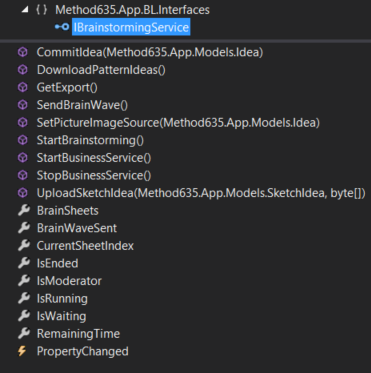
\includegraphics[width=0.5\linewidth]{img/techn-bericht/ibrainstormingservice}
	\caption{Methoden des IBrainstorming-Interfaces}
	\label{fig:ibrainstormingservice}
\end{figure}

Neben diesen erwähnten Services wurden auch Services im Data-Access-Layer (DAL) eingeführt. Diese sind in einem separaten Projekt und können ebenfalls mittels deren Interface in die verwendenden Klassen injiziert werden. Sie sind für den gesamten Daten-Zugriff zuständig. Für das Abbilden der Endpunkte des Backends, wurde weiter ein Konfigurationsfile eingeführt. Dieses Json-File wird geparst und vom \texttt{ConfigurationService} den Repositories zur Verfügung gestellt. 

Für das Einführen von DTOs wurde wie zu Beginn dieses Kapitels erwähnt, dass alle Models in ein separates Projekt ausgelagert wurde. Im DAL existiert ein Ordner mit DTOs, welche für das Parsen der Objekte vom Backend verwendet werden. Es wurde zusätzlich ein Mapping-Layer eingeführt, der die Objekte in die Business Objekte abbildet. Dazu wurde das NuGet-Packet Automapper verwendet. 

Das Auslagern und Zerstückeln der Logik in Services und das Verwenden von Interfaces erleichterte uns die Implementation der nachfolgend beschriebenen Features erheblich. Weiter konnten besonders durch die verschiedenen States in der \texttt{StateMachine} späteres Fehlverhalten viel besser eingeschränkt und korrigiert werden. 

\subsubsection{Implementation Skizzen Feature}
Die Skizzen-Funktion soll es dem Endnutzer ermöglichen, nebst den \texttt{NoteIdeas} auch \texttt{SketchIdeas} (siehe Abbildung \ref{fig:domainmodell-methode635}) zu erfassen. Mit den \texttt{SketchIdeas} wird dem Endnutzer die Möglichkeit gegeben, Skizzen als Teil der Brainstorming-Runden zu zeichnen.

Da es sich bei den einzelnen Skizzen um Binärdaten handelt, musste zunächst eine Möglichkeit geschaffen werden, diese Art von Daten in der Datenbank abzulegen. Dafür wurden in der Elaboration-Phase Analysen (siehe Kapitel \ref{seq:save_file_in_db}) durchgeführt und ein Prototyp erstellt, um die technische Machbarkeit zu verifizieren.

\paragraph*{Implementation Backend}~\\
In den nachfolgenden Listings wird aufgezeigt, wie die Sketch-Funktion im Backend umgesetzt wurde.
Der genaue Kommunikations-Ablauf kann der Abbildung \ref{fig:Seq-Draw-Sketch} in Kapitel \ref{par:sequence-diagramm} entnommen werden.

\begin{lstlisting}[caption={Upload File im File Controller}, label=uploadFileController]
@BodyParser.Of(MultipartFormDataBodyParser.class)
public Result uploadFile(){
    try {

    final Http.MultipartFormData<File> formData = request().body().asMultipartFormData();
    final Http.MultipartFormData.FilePart<File> filePart = formData.getFile("name");
    final File file = filePart.getFile();

    final byte[] fileData = Files.readAllBytes(file.toPath());
    final String fileName = file.getName();

    String fileId = service.uploadFileAsStream(fileData, fileName);
    return ok(Json.toJson(new SuccessMessage("Success", fileId)));

    } catch (IOException | InterruptedException | ExecutionException  e) {
        return internalServerError(Json.toJson(new ErrorMessage("Error", e.getMessage())));
    }
}
\end{lstlisting}

Ähnlich wie bei den JSON-Daten, wird auch hier zunächst die Skizze mittels eines BodyParsers (Zeile 1) in ein File (in-Memory) umgewandelt (Zeilen 5-7), welches dann als Byte-Array dem File-Service (Zeile 12) übergeben werden kann. 

\begin{lstlisting}[caption={Upload File im File Service}, label=uploadFileService]
public String uploadFileAsStream(byte[] stream, String fileName) ... {
    return service.uploadFileAsStream(stream,fileName);
}
\end{lstlisting}

Der File-Service nimmt das Byte-Array entgegen und gibt dieses unverändert dem Datenbank-Service weiter.

\begin{lstlisting}[caption={Upload File im DB Service}, label=uploadFileDBService]
@Override
public String uploadFileAsStream(byte[] stream, String fileName) ... {
    ByteBuffer data = ByteBuffer.wrap(stream);
    CompletableFuture<String> future = new CompletableFuture<>();

    final GridFSUploadStream uploadStream = gridFSBucket.openUploadStream(fileName);
    uploadStream.write(data, (result, t) -> {
        Logger.info("File successfully inserted; ID: " + uploadStream.getObjectId().toHexString());
        future.complete(uploadStream.getObjectId().toHexString());

        uploadStream.close((result1, t1) -> {
            // stream close
        });
    });

    return future.get();
}
\end{lstlisting}

Der Datenbank-Service speichert anschliessend das Bild in die Datenbank (Zeile 7) und liefert bei erfolgreicher Speicherung die ObjektID zurück (Zeile 9). Am Ende wird noch der uploadStream zur Datenbank geschlossen (Zeile 11).

Die Smartphone-Applikation speichert nun die ObjektID als Teil der \texttt{SketchIdea} und sendet das \texttt{Brainsheet} wie gewohnt nach Ablauf der Zeit an das Backend.

Das Herunterladen der gespeicherten Bilder funktioniert auf ganz ähnliche Weise. Da die ObjektID in der \texttt{SketchIdea} abgelegt ist, kann das eigentliche Bild problemlos wiedergefunden werden.

\begin{lstlisting}[caption={Download File im DB Service}, label=uploadFileDBService]
@Override
public byte[] downloadFileAsStream(String id) ...{
    ObjectId fileId = new ObjectId(id);
    final ByteBuffer dstByteBuffer = ByteBuffer.allocate(1024 * 1024);
    final GridFSDownloadStream downloadStream = gridFSBucket.openDownloadStream(fileId);
    CompletableFuture<byte[]> future = new CompletableFuture<>();

    downloadStream.read(dstByteBuffer, (result, t) -> {
        dstByteBuffer.flip();
        byte[] bytes = new byte[result];
        dstByteBuffer.get(bytes);
        Logger.info("Found file to download; Size: " + result);
        future.complete(bytes);

        downloadStream.close((result1, t1) -> {
            // stream closed
        });
    });
    return future.get();
}
\end{lstlisting}

Hierbei wird ein downloadStream geöffnet, welcher die Daten anhand der ID aus der Datenbank liest und in ein Byte-Array schreibt (Zeile 8). Auch hier wird am Ende der Stream wieder geschlossen (Zeile 15).

Der zurückgelieferte Byte-Array wird anschliessend unverändert an den Client zurück\-geschickt. Allfällige Fehler während der Ausführung sowohl beim Hochladen wie auch beim Herunterladen werden im File-Controller abgefangen und als Fehler an den Client geschickt.

\paragraph*{Implementation Frontend}~\\
%TODO Sketch beschreiben

\subsubsection{Implementation Pattern Feature}
Nebst der Skizzen-Funktion war es unser Ziel, dem Endnutzer eine Funktion anzubieten, welche es ihm ermöglicht, aus einer Liste von verschiedensten Pattern ein passendes Pattern auszuwählen. 

Wir erweiterten unsere Applikation daher um eine \texttt{PatternIdea}. Die verwendeten Pattern stammen ausschliesslich von der Webseite \href{https://microservice-api-patterns.org}{Microservice API Patterns}. Dabei ist es aber durchaus auch denkbar Pattern von anderen Quellen zu nehmen oder sich gar auf nicht-software Pattern zu konzentrieren.

\paragraph*{Implementation Backend}~\\
In den nachfolgenden Listings wird aufgezeigt, wie die Pattern-Funktion im Backend umgesetzt wurde.
Der genaue Kommunikations-Ablauf kann der Abbildung \ref{fig:Seq-Insert-Pattern} im Kapitel \ref{par:sequence-diagramm} entnommen werden.

\begin{lstlisting}[caption={Alle Pattern holen im Pattern Controller}, label=getAllPatternInController]
 public Result getAllPatternIdeas(){
    CompletableFuture<Queue<PatternIdea>> future = service.getAllPatternIdeas();
    ArrayList<JsonNode> list = new ArrayList<>();

    try {

        for (PatternIdea patternIdea : future.get()) {
            PatternIdeaDTO patternIdeaDTO = modelsMapper.toPatternIdeaDTO(patternIdea);
            JsonNode node = Json.toJson(patternIdeaDTO);
            ((ObjectNode)node).put("type", "patternIdea");
            list.add(node);
        }

        return ok(Json.toJson(list));

    } catch (InterruptedException | ExecutionException e) {
        return internalServerError(Json.toJson(new ErrorMessage("Error", e.getMessage())));
    }
}
\end{lstlisting}

Um alle verfügbaren Pattern abzurufen wird auf dem Pattern-Service (Zeile 2) die Methode \textit{getAllPatternIdeas} aufgerufen. Anschliessend werden die gefundenen Pattern lediglich in ein DTO umgewandelt (Zeile 8) und fast unverändert als JSON an den Client gesendet (Zeile 14).

Der Endnutzer kann nun aus einer Liste der verfügbaren Pattern das gewünschte Pattern auswählen. Dieses wird, wie schon die \texttt{SketchIdea} oder \texttt{NoteIdea}, als Teil des \texttt{Brainsheets} an das Backend geschickt. 

Wie in allen Controller-Klassen werden auch hier allfällige Fehler während der Ausführung abgefangen und an den Client gesendet (Zeile 16/17).

\begin{lstlisting}[caption={Alle Pattern holen im Pattern Service}, label=getAllPatternInService]
public CompletableFuture<Queue<PatternIdea>> getAllPatternIdeas(){
        return service.getAllPatternIdeas();
}
\end{lstlisting}

Der Pattern-Service leitet den Aufruf seinerseits direkt an den Datenbank-Service weiter.

\begin{lstlisting}[caption={Alle Pattern holen im Pattern DB Service}, label=getAllPatternInDBService]
@Override
public CompletableFuture<Queue<PatternIdea>> getAllPatternIdeas() {
    CompletableFuture<Queue<PatternIdea>> future = new CompletableFuture<>();
    Queue<PatternIdea> queue = new ConcurrentLinkedQueue<>();

    patternIdeaCollection.find().sort(Sorts.ascending("category")).forEach(
            finding -> queue.add(finding), (result, t) -> {
                Logger.info("Get all available patterns");
                future.complete(queue);
            });

    return future;
}
\end{lstlisting}

Der DB-Service wiederum findet alle Pattern und gibt diese nach Kategorie sortiert (Zeile 6-12) als Resultat zurück.

\paragraph*{Implementation Frontend}~\\
%TODO Pattern beschreiben

\subsubsection{Implementation Export Feature}
Die letzte Funktion, welche wir in unserer Bachelorarbeit verwirklichen wollten, war die Möglichkeit, die erarbeiteten Lösungsvorschläge in geeigneter Form zu exportieren.

Nach einer kleineren Analysephase und einer Beratungsrunde mit unserem Betreuer fiel die Wahl nach der geeigneten Form auf Markdown \cite{markdown}. Der Vorteil von Markdown sahen wir vor allem darin, dass man Markdown schnell und einfach z.B. auf GitHub hochladen kann. Da man als Entwickler tendenziell viel mit GitHub oder ähnlichen Tools/Webseiten arbeitet, empfanden wir diese Umsetzung am  einfachsten und intuitivsten von der Handhabung.

\paragraph*{Implementation Backend}~\\
Die Möglichkeit des Exports wird hauptsächlich durch das Backend bereit gestellt. Dabei wurden die Business-Objekte um eine Serialize-Methode erweitert, welche beschreibt, wie die Objekte im Markdown aussehen sollten bzw. welche Informationen wie (Text, BoldText, ItalicText, Header, etc.) dargestellt werden sollten. 

In den nachfolgenden Listings wird aufgezeigt, wie die Export-Funktion und die Serialize-Methode im Speziellen für das \texttt{BrainstormingFinding} im Backend umgesetzt wurde. Die Umsetzung für die anderen Business-Objekte ist entsprechend gleich aufgebaut. 

\begin{lstlisting}[caption={Serialize-Methode von BrainstormingFinding}, label=markdownBrainstormingFinding]
public class BrainstormingFinding implements MarkdownCascadable {
...
public String getPredecessor() {
    return new Heading(getName(),1).toString() + "\n";
}

...
public String getSuccessor() {
    StringBuilder successor = new StringBuilder();

    successor.append(new BoldText("Basic Information").toString()).append("\n")
    .append(new Text("Description: ").toString())
    .append(getProblemDescription()).append("\n")
            ...
    return successor.toString();
}

...
public String serialize() throws MarkdownSerializationException {

    if (getName().equals("") || getNrOfIdeas() == 0 || getType().equals("") || getBrainstormingTeam().equals("")) {
        throw new MarkdownSerializationException("name is null or description");
    }

    StringBuilder brainsheets = new StringBuilder();

    for (Brainsheet brainsheet: getBrainsheets()){
        brainsheets.append(brainsheet.serialize());
    }
    
    return getPredecessor() + getSuccessor() + brainsheets.toString();
	}
}

\end{lstlisting}

Im \textit{FindingController} wird nun die \texttt{exportBrainstorming}-Methode auf dem Business-Service aufgerufen (Zeile 3).

\begin{lstlisting}[caption={Export-Methode im FindingController}, label=markdownFindingController]
public Result exportBrainstorming(...){
try {
String result = service.exportBrainstorming(findingIdentifier);

    if (result != null) {
        return ok(result);
    } else {
        return badRequest(...);
    }
    
} catch (InterruptedException | ... e) {
    return internalServerError(Json.toJson(new ErrorMessage("Error", e.getMessage())));
}
}
\end{lstlisting}

Der Business-Service wiederum holt das \textit{BrainstormingFinding} (Zeile 2) und das \textit{BrainstormingTeam} (Zeile 5), setzt statt der Team-ID den Namen des Teams (Zeile 6) und führt am Ende die erwähnte Serialize-Methode aus (Zeile 7). 

\begin{lstlisting}[caption={Export-Methode im FindingService}, label=markdownFindingService]
public String exportBrainstorming(String findingIdentifier) ...{
BrainstormingFinding finding = service.getFinding(findingIdentifier).get();

if (finding != null) {
    BrainstormingTeam team = teamService.getTeam(finding.getBrainstormingTeam()).get();
    finding.setBrainstormingTeam(team.getName());
    return finding.serialize();
}

return null;
}
\end{lstlisting}

Die Tatsache, dass wir neben unseren Business-Objekten sogenannte DTOs in unsere Applikation integrierten, konnte in dieser Funktion gut ausgenutzt werden. So wurde die Serialize-Methode lediglich in den Business-Objekten implementiert, da sie einen Bestandteil der Business-Logik darstellt und weniger essenziell für die Kommunikation ist.

\paragraph*{Implementation Frontend}~\\
%TODO Export beschreiben

\subsubsection{Verwendete Bibliotheken im Backend}
Tabelle \ref{tab:verwendete-libraries-play} zeigt die Bibliotheken auf, die im Backend verwendet werden. 
\begin{table}[h]
	\centering
	\begin{tabular}{| l | l | c | l |}
		\hline
		\textbf{Bibliothek} & \textbf{Version} & \textbf{Repository} & \textbf{Lizenz}\\
		\hline
		swagger-play2 & 1.6.0 & \href{https://mvnrepository.com/artifact/io.swagger/swagger-play2_2.12/1.6.0}{mvnrepository.com} & Apache 2.0 \\
		java-jwt & 3.2.0 & \href{https://mvnrepository.com/artifact/com.auth0/java-jwt/3.2.0}{mvnrepository.com} & MIT \\
		mongodb-driver-async & 3.8.0 & \href{https://mvnrepository.com/artifact/org.mongodb/mongodb-driver-async/3.8.0}{mvnrepository.com} & MIT \\
		modelmapper & 2.3.2 & \href{https://mvnrepository.com/artifact/org.modelmapper/modelmapper/2.3.2}{mvnrepository.com} & Apache 2.0 \\
		markdowngenerator & 1.3.1.1 & \href{https://mvnrepository.com/artifact/net.steppschuh.markdowngenerator/markdowngenerator}{mvnrepository.com} & Apache 2.0 \\
		\hline
	\end{tabular}
	\caption[Story-Points]{Verwendete Bibliotheken Backend}
	\label{tab:verwendete-libraries-play}
\end{table}

\subsubsection{Verwendete Bibliotheken im Frontend}
In Tabelle \ref{tab:verwendete-libraries-frontend} sind die verwendeten Libraries und Frameworks des Frontends aufgelistet.
\begin{table}[!h]
	\centering
	\begin{tabular}{| l | l | c | l |}
		\hline
		\textbf{Bibliothek} & \textbf{Version} & \textbf{Repository} & \textbf{Lizenz}\\
		\hline
		CarouselView.FormsPlugin & 5.2.0 & \href{https://github.com/alexrainman/CarouselView}{github.com} & MIT \\
		Microsoft.AppCenter & 1.10.0 & \href{https://visualstudio.microsoft.com/app-center/}{AppCenter} & MIT \\
		NUnit & 3.11.0 & \href{http://nunit.org}{nunit.org} & MIT\\
		NUnit3TestAdapter & 3.11.2 & \href{https://github.com/nunit/docs/wiki/Visual-Studio-Test-Adapter}{github.com} & MIT\\
		Prism.Forms & 7.0.0.396 & \href{https://github.com/PrismLibrary/Prism}{github.com} & MIT \\
		Xamarin.Forms & 3.3.0.912540 & \href{https://docs.microsoft.com/en-us/xamarin/xamarin-forms/}{Microsoft Docs} & MIT \\
		XamlStyler.Console & 3.0.0 & 
		\href{https://github.com/Xavalon/XamlStyler}{github.com} & Apache 2.0\\
		ZXing.Net.Mobile & 2.4.1 & \href{http://github.com/Redth/ZXing.Net.Mobile}{github.com} & Apache 2.0\\
		ZXing.Net.Mobile.Forms & 2.4.1 &
		\href{http://github.com/Redth/ZXing.Net.Mobile}{github.com} & Apache 2.0\\
		\hline
	\end{tabular}
	\caption{Direkt verwendete Bibliotheken Frontend}
	\label{tab:verwendete-libraries-frontend}
\end{table}


\subsubsection{Vergleich Soll/Ist}
Wie aus dem Projektplan (siehe Kapitel \ref{subsec:timeline}) zu entnehmen ist, nahmen wir uns für die Zeit während der Construction vor, ein Refactoring durchzuführen und die Skizzenfunktion (Use-Case 8c), die Patternfunktion (Use-Case 8e) sowie die Exportfunktion (Use-Case 13) zu implementieren. 

Obwohl das Refactoring etwas mehr Zeit als zunächst gedacht benötigte, konnten wir die gesetzten Ziele allesamt erreichen. Die restlichen drei Use-Cases aus dem Kapitel \ref{par:fully-dressed-uc} waren für uns schon von Beginn weg niedriger priorisiert. Dies aus dem Grund, da diese keine businesskritische Funktion darstellten bzw. durch die anderen Use-Cases teilweise abgedeckt werden konnten (Links können z.B. auch als normaler Text eingegeben werden). Weitere nicht implementierten Features sind: Use-Case 2: Logout auf Back- und Frontend sowie Use-Case 4: Delete Account und Use-Case 6: Leave Brainstorming Team auf dem Frontend. Da wir uns auf die oben erwähnten Arbeiten konzentrieren, war es auch nie ein definiertes Ziel dieser Arbeit, diese umzusetzen. 

Die Ziele aus der Aufgabenstellung (siehe Anhang \ref{sec:aufgabenstellung}) wurden wir folgt erreicht. Die Erweiterbarkeit ist durch die Applikation gegeben. Wie im Anhang \ref{sec:Ideen_Erweiterung} beschrieben, ist es ohne grosse Aufwände möglich, die bestehende Applikation um weitere Ideen-Typen zu erweitern. Auch steht der Integration von anderen Brainstorming- und Innovationsmethoden nichts im Wege.

Auch die Ausnutzung der Smartphone-Fähigkeiten bzw. die Verwendung der verschiedenen Medien wurde erweitert. Dank des Touchscreen ist es z.B. möglich Skizzen zu zeichnen. Die Patternfunktion ermöglicht es zudem ein vordefiniertes Pattern als weiteres, neues Medium zu nutzen.

Das Ziel der einfachen und intuitiven Bedienung der App, einem unkomplizierten Reporting sowie der Robustheit und der Stabilität der App konnten dank den durchgeführten User-Tests validiert und beurteilt werden. Die Resultate dazu finden sich in den Kapitel \ref{subsec:ergebnisbewertung} und \ref{subsec:testauswertung}.